\documentclass[11pt]{report}

% I want multiple citations to be condenced. ie. [1, 2, 3, 4] -> [1-4]
% I want back references in my bibliography.
\usepackage[backref = true, sorting = none, backend = bibtex, style=nature]{biblatex}
% Phrase the back reference nicely.
\DefineBibliographyStrings{english}{%
  backrefpage = {cited on page},
  backrefpages = {cited on pages},
}
% Links without boxes around them.
\usepackage[hidelinks]{hyperref}
% Color for... color.
\usepackage{color}
% Need this for figures
\usepackage{graphicx}
% This may include the bibliography in the table of contents
\usepackage[numbib]{tocbibind}
% Slightly neater way of doing units.
\usepackage{units}
% Glossary package for acronyms.
\usepackage[nonumberlist]{glossaries}%[nonumberlist,nohypertypes={glossary},acronym]
\setglossarysection{subsubsection} % No page break on \printglossary
\renewcommand{\glossarysection}[2][]{} % No glossary title.

\include{acronyms}
\makeglossaries

% Add the .bib file.
\bibliography{Library}

\begin{document}

% Title page
\title{Thesis}

\author{Joshua Torrance}

\pagenumbering{alph} % Title page becomes a so backrefs to 1 go to the right place.
\maketitle

\pagenumbering{roman}

% Front matter
\chapter*{Abstract}
\addcontentsline{toc}{chapter}{Abstract}

The understanding of atomic structures and processes is continually improving with the great technological development in imaging techniques.
Ultrafast electron and X-ray techniques are able to perform measurements at atomic lengths and timescales and both these techniques require the generation of high-brightness ultrashort-duration electron bunches.
Electron imaging techniques directly use these short bright bunches and in \glspl{xfel} the electron bunches are used to generate short bright bunches of X-rays.

It is hoped that \glspl{caeis} will also be able to produce ultrashort high-brightness electron bunches that are brighter than conventional sources.
\Glspl{caeis} generate electrons via near-threshold ionisation from an ultracold atomic gas and have been shown to create electrons bunches with temperature as low as \unit[10]{K}.
Conventional photocathode sources have temperatures of thousands of Kelvin and, as brightness is proportional to the temperature of the source, \glspl{caeis} have the potential to produce much brighter electron bunches.
\Gls{caeis} are also capable of producing extremely cold ion bunches and show great promise as an ion source for ion milling and microscopy.

This thesis describes a number of developments involved with the \gls{caeis} project at the University of Melbourne, in particular pushing the boundaries of laser frequency stabilisation to allow for precise selection of atomic states for cooling and ionisation, and a new technique for measuring the brightness of charged particle bunches.

Laser frequency stabilisation is an essential component of the \gls{caeis} and many other applications including metrology, spectroscopy and laser cooling.
Polarisation spectroscopy is a commonly used technique for laser frequency stabilisation but the full measurement and control bandwidth has not previously been demonstrated.
Here it is shown that the bandwidth is sufficient to not only stabilise the frequency of the laser, but also to reduce the laser linewidth to much less than \unit[1]{kHz}, two order, two orders of magnitude better than previously reported.
This demonstration provides a new approach for precisely accessing the high-lying Rydberg-levels of atoms, if used in conjunction with cavity based frequency locking methods, allowing for a greater exploration of the ionisation methods involved in a \gls{caeis}.

Brightness is the most comprehensive figure of merit for charged particle beams and a new technique for measuring the brightness with sub-nanosecond time-resolution is presented.
The technique achieves time-resolved brightness measurements by streaking one-dimensional pepperpot measurements across the detector.
Time-resolved brightness measurements have the potential to reveal information related to the ionisation processes used in \glspl{caeis} and can show the efficacy of techniques used to counter the effects of space charge in the beams produced from a \gls{caeis}.

The performance of the \gls{caeis} apparatus operating in its normal pulsed mode is compared to continuous operation with emphasis on the beam current and electron trajectory stability.
The beam quality was also improved by identifying an astigmatism in the beam and correcting it with a 3D printed quadrupole lens.
Virtually all the beam measurements presented here utilise image processing techniques that allow for multi-shot averaging despite instabilities in the electron beam trajectories.

This iteration of a \glspl{caeis} was able to produce ultrashort-duration electron bunches and these have been used to demonstrate ultrafast electron diffraction from thin gold foils.
This is an important step along the path to being able to perform ultrafast single-shot \gls{cdi} and the next iteration of the \gls{caeis} should have sufficient current to demonstrate diffraction that is both single-shot and ultrafast.
\chapter*{Acknowledgements}
\addcontentsline{toc}{chapter}{Acknowledgements}

Acknowledgements go here.

\chapter*{Contributions}
\addcontentsline{toc}{chapter}{Contributions}

List of contributions go here.


\tableofcontents

\chapter{Introduction}
 
\pagenumbering{arabic}
\setcounter{page}{1}

Molecular imaging has provided science with great advances, such as the determination of the helical structure of DNA in 1953~\cite{watson_molecular_1953}, and the discovery of the structure of myoglobin and haemoglobin in 1962~\cite{kendrew_x-ray_1957}.
The \gls{caeis} at the University of Melbourne is an ongoing project that aims to develop a source capable of achieving the `holy grail' of scientific imaging, the \emph{molecular movie}~\cite{dwyer_femtosecond_2006,sciaini_femtosecond_2011}.
A \gls{caeis} also has enormous potential for ion beam technologies such \glspl{fib}~\cite{mcclelland_bright_2016}, ion microscopes~\cite{knuffman_cold_2013}, and as a source for accelerators such as synchrotrons and \glspl{xfel}~\cite{van_oudheusden_electron_2007,zhu_future_2015,mcculloch_cold_2016}.
Depending on the context a \gls{caeis} is also sometimes referred to as a \gls{caes} or \gls{cais}.

\section{Making the `Molecular Movie'}

The ability to observe molecular dynamics at an atomic spatial and temporal scale could provide great insight into some of the basic processes of biology and chemistry.
The fabled `molecular movie' refers to capturing the atomic motions of molecular systems with atomic-scale spatial resolution as they undergo some transition such as a chemical reaction, protein folding, melting, or even just atomic vibrations.
Molecular movies could provide greater understanding of important biological reactions such as photosynthesis or oxygen transport by haemoglobin.

One of the stepping stones towards molecular movies is single-shot imaging of non-crystalline molecules which would allow structural determination of membrane proteins, an essential step in rational drug design~\cite{hardy_atomic_1987, barrett_discovering_1999, pinto_influenza_1992}.
The majority of imaging performed to date has been on crystalline targets and the related imaging techniques are much better developed than those for non-crystalline targets.
One of the main techniques in structural determination of crystalline targets is electron diffraction which, along with X-ray and neutron methods~\cite{cullity_elements_2001,bacon_x-ray_2013}, has been utilised in structural determination of many materials with atomic resolution.
Continuing research into real-space and diffraction imaging techniques is aiding in the understanding of a growing range of samples as well as providing new types of information on the samples under investigation.

In the past the greatest success with structural determination has been achieved with crystallography, limited to samples that can be crystallised.
There are a large number of biological proteins of interest, particularly membrane proteins, that cannot be crystallised and developments in ultrafast imaging techniques are providing a route towards structural determination without crystallisation~\cite{dauter_current_2006,levitt_nature_2009}.
Cryogenic electron microscopy is also making headway in this area but is unable to measure dynamics~\cite{henderson_model_1990,zhou_towards_2008}.
Ultrafast imaging techniques are a relatively recent development and they provide the opportunity to study electronic and atomic dynamics.
Ultrafast techniques allow for imaging to be completed before damage to the sample from the illumination makes imaging impossible~\cite{gaffney_imaging_2007,barty_ultrafast_2008,miao_beyond_2015}.
Both X-ray and electron imaging techniques are limited by the capabilities of their sources which are undergoing continual development.
The techniques using X-rays and electrons each have different advantages and disadvantages with regards to dynamic imaging and structural determination and they often give complementary information.

One proposed method for generating molecular movies involves using a high-brightness ultrashort duration beam source, such as an \gls{xfel} or future \gls{caes}, to perform \gls{cdi} on individual molecules~\cite{chapman_femtosecond_2006,dwyer_femtosecond_2006,gaffney_imaging_2007}.
The individual molecules would be dropped one-by-one in front of the illuminating bunches which would be short enough that imaging is completed before damage from the illumination affects the diffraction pattern (see Figure~\ref{figure:molecule_cdi}).
Dynamic processes, such as phase transitions, melting, and pumped vibrational modes, can be studied with this technique if the process can be triggered, say with a precisely timed laser pulse.
By varying the delay between triggering the process and imaging a `movie' can be constructed.
The random orientation of molecules as they are imaged can be managed algorithmically as long as there is sufficient brightness with each shot~\cite{yefanov_orientation_2013}.

\begin{figure}
    \center
    \includegraphics[width=0.65\linewidth]{0intro/Figs/single_molecule_cdi.jpg}
    \caption[Structural determination of single molecules.]{Structural determination of single molecules should be possible if a sufficiently bright and short pulse of X-rays is used image the molecule before damage affects the diffraction pattern produced. Electrons could be used in place of X-rays if a suitable source can be developed. Image adapted from Reference~\cite{gaffney_imaging_2007}}
    \label{figure:molecule_cdi}
\end{figure}

\Glspl{xfel} have been able to produce molecular movies~\cite{kupitz_structural_2016,pande_femtosecond_2016,nango_three-dimensional_2016} but there is still motivation for attempting to develop electron source alternatives.
Electrons interact much more strongly with matter than X-rays, with interactions having cross-sections $10^5$ to $10^6$ larger~\cite{sciaini_femtosecond_2011} and thus much fewer electrons are required per bunch than X-ray photons.
While \glspl{xfel} require a several kilometre long facility with a billion dollar price tag a hypothetical electron source with similar capabilities would likely fit in a room with a much lower cost: current \gls{caes} implementations easily fit on a single optical bench.

\subsection{Ultrafast Coherent Diffractive Imaging}

Resolving the structure of single molecules requires sufficient signal such that the orientation problem can be solved and averaging performed, and the imaging needs to be completed before the molecule is substantially damaged by the beam~\cite{huldt_diffraction_2003}.
Thus a single pulse must be extremely intense, in one scenario requiring $10^{12}$ \unit[8]{kV} X-ray pulses or $10^6$ \unit[3]{MeV} electrons, and extremely short in duration, 10s of femtoseconds~\cite{chapman_femtosecond_2006,spence_outrunning_2017}.
Damage to molecules can occur via numerous mechanisms and are different for X-rays and electrons but in both cases occur in approximately 10s of femtosecond timescales~\cite{spence_outrunning_2017}.

The coherence of the source is also an important consideration for diffraction imaging as the beam must have a coherence length as large as that of the molecule under consideration so that portions of the illuminating wave diffracted from different positions on the molecule interfere coherently.
When performing \gls{cdi} the diffraction pattern detected is the square of the Fourier coefficients that represents the molecule under examination.
Due to the loss of the complex phase components when the Fourier coefficients are squared it is not possible to directly invert to recover the structure of the molecules, this is known as the \emph{phase problem}~\cite{rodenburg_phase_1989}.
The most common solution to the phase problem is iterative computational phase-retrieval~\cite{chapman_coherent_2010}.

Ultrafast \gls{cdi} has been demonstrated has been demonstrated previously on micron-scale objects using an \gls{xfel}~\cite{chapman_femtosecond_2006}.

\subsection{Imaging Targets}

Crystallography has been of enormous benefit to biology as the structure of biological molecules plays a vital role in their function, with proteins interacting with sub-structures of other proteins to mediate biological processes, somewhat analogous to a lock and key or jigsaw pieces.
Knowing the structure of biological proteins is essential to fully understanding how the mechanism that protein is involved in functions and can provide vital information to researchers on how to produce drugs to manipulate that mechanism~\cite{aloy_structural_2006,almen_mapping_2009}.
The design and creation of drugs based on knowledge of the structure of the proteins involved in a mechanism is sometimes referred to as \emph{direct drug design} and has had some success to date~\cite{klebe_recent_2000,jhoti_structure-based_2007,mauser_recent_2008}.
The first example of structurally informed direct drug design was the drug dorzolamide which was released to the market in 1995 to reduce intraocular pressure in certain circumstances~\cite{greer_application_1994}.

One of the obvious restrictions on crystallography is that the target sample must be crystallisable in order for it to be imaged and unfortunately there are large numbers of important biological proteins that scientists have been unable to crystallise, notably a large portion of membrane proteins which mediate interactions on the surfaces of cells~\cite{geerlof_impact_2006}.
Alternative structure determination techniques such as ultrafast \gls{cdi} with an \gls{xfel} or \gls{caes} would be able to bypass the crystallisation requirement and thus provide researchers with a wealth of useful information.

Knowledge of the changes in molecular structures during many complex and interesting dynamics (such as melting, photosynthesis, molecular phase transitions, or chemical reactions) would prove invaluable to understanding the physics, chemistry and biology of many areas.

\section{Cold-atom electron and ion sources}

The research described by this thesis is part of an ongoing effort to develop an alternative source of electrons and ions that extracts the charged particles from a laser cooled atomic cloud.
Initially the aim of the project was to create ultrafast coherent electron bunches for use in diffraction imaging in a similar way to ultrafast X-ray pulses however it was later realised that \gls{caes} could also serve as an injection source for particle accelerators.
It has also become apparent that by simply reversing the polarity of the accelerator the source can generate high quality ion bunches with similar properties to the electron bunches thus providing a new source for use in ion microscopy and nano-fabrication.

Cold-atom sources operate by carefully ionising atoms in a \gls{mot} such that the resulting ions and electrons are cold and thus the bunches accelerated from those clouds have low emittance and high coherence.
A brief schematic of \gls{caeis} operation is shown in Figure~\ref{figure:simple_caeis_schem}.
The low transverse temperature of ions and electrons produced by a \gls{caeis} is one of the main advantages of this source.
The source also allows for the production of ultrafast, and arbitrarily shaped electron and ion bunches.
These techniques are applicable to any of the many atomic species that can be laser cooled and trapped.

\begin{figure}
    \center
    \includegraphics{0intro/Figs/simple_caeis_schem.pdf}
    \caption[Simplified cold atom ion and electron source schematic.]{Rubidium atoms are trapped and cooled in a \gls{mot} before being ionised with a red and blue laser. The electrons or ions are then accelerated by two electrodes forming the electron or ion bunches. In this diagram the blue ionisation laser comes from behind the atom cloud.}
    \label{figure:simple_caeis_schem}
\end{figure}

A \gls{caes} can be thought of as a photocathode electron source with the solid cathode replaced with an ultracold gas which provides the \gls{caes} with a few advantages such as high quantum efficiency, and near-threshold ionisation producing colder electrons than those from other photocathode sources~\cite{engelen_effective_2014}.
The simplicity of the interactions between photons and atoms allows for the high quantum efficiency to be achieved~\cite{baranov_field_1994}.

Another advantage of gas photocathodes is the lack of optically induced damage from high-intensity laser-fields.
Solid cathodes undergo constant degradation and require regular replacement~\cite{dowell_results_1995} whereas the gaseous target in a \gls{caes} is renewed with every bunch produced.

A major advantage of \glspl{caeis} as a electron or ion source is the low temperature of the source.
The low source temperature is due to the careful ionisation of the atoms trapped within the \gls{mot}.
The ultracold atoms trapped in the \gls{mot} have temperatures around \unit[100]{$\muup$K} but after ionisation the electrons have temperatures determined by the excess energy from the ionisation process~\cite{engelen_high-coherence_2013,engelen_analytical_2014,sparkes_high-coherence_2014,speirs_identification_2017}.
Precise control over the ionisation allows the excess energy from the ionisation process to be minimised and the electrons produced can have transverse temperature as low as \unit[$\sim$10]{K}~\cite{saliba_spatial_2012}.
Unlike electrons, ions produced by the source have their initial temperature determined predominantly by the temperature of the trapped atoms before ionisation, \unit[100]{$\muup$K}, with an ion temperature around \unit[1]{mK}~\cite{debernardi_measurement_2011,murphy_detailed_2014}.

The ionisation methods used in \glspl{caeis} involve a two-step ionisation process that first excites the atoms to an intermediate state with one laser followed by near-threshold ionisation of the excited atoms with a second laser frequency-tuned to minimise the excess ionisation energy.
Generally the second stage in the excitation process involves exciting the atom from the intermediary excited state to a high-lying Rydberg state from which the atom can be field ionised in the presence of the accelerating electric field~\cite{mcculloch_field_2017}.
Due to the small energy difference between high-lying Rydberg states narrow linewidth lasers are required and in order to provide such lasers the limits of polarisation spectroscopy~\cite{wieman_doppler-free_1976} as a laser frequency stabilisation technique have been explored in Chapter~\ref{chapter:polspec}~\cite{torrance_sub-kilohertz_2016}.
Polarisation spectroscopy with high-bandwidth feedback is able to provide laser frequency linewidths two orders of magnitude smaller that those previously reported and this will prove useful for precision interaction with the high-lying Rydberg levels used in \gls{caeis} ionisation as well as other fields such as spectroscopy or metrology where low laser linewidth is important.

The sophisticated ionisation scheme used in a \gls{caeis} allows for the production of ultrashort duration bunches and arbitrary shaping of the bunches.
\Glspl{caeis} have been shown to be able to produce electron bunches with duration less than \unit[130]{ps} (with expected bunch duration of a few tens of picoseconds)~\cite{speirs_identification_2017} and should be able to provide bunches suitable for compression to bunch duration of order \unit[100]{fs}, suitable for ultrafast imaging~\cite{van_oudheusden_compression_2010}.

\Glspl{caeis} also have the ability to produce arbitrarily shaped electron or ion bunches by manipulating the profiles of the laser beams used to ionise the atoms~\cite{mcculloch_arbitrarily_2011}.
This capability is useful in a large number of ways but has particular potential as an avenue for production of uniform ellipsoidal to allow for reversal of beam-quality degradation by space-charge expansion~\cite{luiten_how_2004,thompson_bunch_2015}.

One of the most important figures of merit for charged particle beam is beam emittance which can be directly correlated with the temperature of the particle source.
Emittance describes the angular spread of particles within a beam or bunch and can be thought of as the ``focusability of the beam'' with low-emittance being preferable to high-emittance.
Due to the extremely low temperature \glspl{caeis} have enormous potential as a source for low-emittance electron and ion bunches.
Low-emittance is also related to high-coherence which is a vital consideration for imaging.
The coherence length of a source must be at least as large as that of the sample under consideration for techniques such as \gls{cdi} or at least as large as the unit cell length for crystallographic diffraction techniques.
\Glspl{caeis} have already demonstrated impressive coherence lengths as large as those of some small biomolecules with further improvements expected~\cite{saliba_spatial_2012}.

A new technique for measuring beam brightness (a metric that combines beam emittance and current) with time-resolution was developed which operates by streaking one-dimensional pepperpot measurements across the detector~\cite{torrance_time-resolved_2018}, see Chapter~\ref{chapter:brightness}.
This method was developed to allow for examination of the efficacy of space-charge reversal techniques when they are implemented with a \gls{caeis} and to learn more about the ionisation processes involved in a \gls{caeis}.
This technique is generally applicable to charged particle beams, not just \glspl{caeis}, and could prove useful in numerous applications.

\Glspl{caes} have been used to demonstrate single-shot diffraction~\cite{speirs_single-shot_2015} and ultrafast diffraction (see Chapter~\ref{chapter:diffraction}) from gold nanofilm.
To-date diffraction that is both single-shot and ultrafast has not been achieved due to the low beam current of this \gls{caes} implementation but there are a number of strategies that may be able to improve on this, some of which are explored in Chapter~\ref{chapter:setup}.
If the beam current of \glspl{caes} can be improved then there is enormous potential for the source as it will produce high-brightness, ultrashort-duration electron bunches with strategies available to counter the effects of space-charge expansion.
\Glspl{caes} show great promise as a source for \gls{cdi} and the production of molecular movies.

\subsection{Ion Source}

By reversing the polarity of the acceleration stage of beam production in a \gls{caeis} a beam of ions can be produced instead of an electron beam.
Ion beams share the same advantages as the electron beams with bunches being shapeable, coherent and low-emittance~\cite{knuffman_cold_2013}.

\glsreset{fib}
\Glspl{fib} have a wide variety of applications such as high-resolution imaging~\cite{scipioni_helium_2008}, sample analysis and nanofabrication~\cite{khizroev_focused-ion-beam-based_2004}.
Liquid metal ion sources are the most commonly used \gls{fib} sources, usually using gallium ions due to it's simplicity and robustness despite gallium having a tendency to contaminate or destroy samples.
\Glspl{cais} promise to provide an attractive alternative to conventional sources as they have high-brightness, low-emittance and are able to operate with a large range of ions, which could be selected to avoid sample contamination.

\Glspl{cais} have been used to demonstrate microscopy with lithium ions~\cite{knuffman_nanoscale_2011} and chromium ions~\cite{steele_focused_2010}.
Rubidium \gls{cais} ion beams have been characterised and used to demonstrate the suppression of space-charge expansion~\cite{murphy_detailed_2014,thompson_suppression_2016}.

\section{Summary}

Molecular structural determination of biological proteins is an essential component of modern developments in medicine and new tools are constantly required to allow the boundaries of this field to be pushed back.
\Glspl{caes} have great potential as an alternative source for molecular imaging and may one day be able to challenge existing sources such as \gls{xfel}, photocathode electron sources, and cryoelectron microscopes.
Current \glspl{caes} are able to produce high-brightness, ultrashort-duration bunches with coherence lengths equal to that of small biomolecules and if the beam current can be improved on in the next generation of \gls{caes} then they will be well on the way to becoming a competitive source for the production of molecular movies.

\Glspl{caeis} operating in ion mode also show much promise in \gls{fib} applications.
\Gls{cais} technology may well be applicable to any atom that can be optically trapped which will provide significantly more scope to the application of \glspl{fib}.

This thesis discusses the implementation of the \gls{caeis} located at the University of Melbourne that operated until 2018 and the continuous characterisation and improvement it underwent (Chapter~\ref{chapter:setup}), research that was able to improve the performance of polarisation spectroscopy as a frequency stabilisation technique to demonstrate sub-kilohertz linewidth (Chapter~\ref{chapter:polspec}), diffraction results from the \gls{caes} demonstrating ultrafast diffraction from gold foil (Chapter~\ref{chapter:diffraction}), and a new method for measuring time-resolved emittance by streaking one-dimensional pepperpots (Chapter~\ref{chapter:brightness}).

% The following two lines need to be in the first chapter to get Arabic page numbers.
%\pagenumbering{arabic}
%\setcounter{page}{1}
\part[Polarisation Spectroscopy]{Polarisation Spectroscopy\\
\vspace{1cm}
\LARGE Pushing the Limits of Polarisation Spectroscopy as a Laser Frequency Reference}
\chapter{Introduction}

Laser frequency stabilisation is an essential tool for atomic physics experiments, without it experiments involving \glspl{bec}, atomic clocks and many more would not be possible~\cite{anderson_observation_1995,ye_quantum_2008}.
There are a plethora of techniques available for laser frequency stabilisation each with numerous advantages and disadvantages.

\Gls{ps} is one such technique that will be discussed in detail~\cite{demtroder_laser_2003}.
\Gls{ps} was first described by Wieman and H\"anch in 1976 as, ``...a sensitive new method of Doppler-free spectroscopy, monitoring the nonlinear interaction of two monochromatic laser beams in an absorbing gas via changes in light polarisation."~\cite{wieman_doppler-free_1976}
This chapter provides an overview of laser frequency stabilisation, a detailed discussion of the physics of \gls{ps} followed by details on the implementation and measurement of high bandwidth frequency stabilisation using \gls{ps}.

\section{Laser Frequency Stabilisation}

Laser frequency stabilisation describes a number of techniques that are used to reduce the temporal frequency spread of a laser's frequency.
This can range from weak frequency stabilisation keeping the centre frequency of a laser at a particular point to convoluted frequency narrowing techniques that attempt to reduce laser linewidth to sub-hertz levels.
Typically these techniques use some reference to measure frequency deviation from a given frequency and provide negative feedback to the laser, using a servo system, to keep it at the target frequency.

The efficacy of stabilisation techniques can be described by width of the frequency distribution of the laser, called the linewidth.
Width is usually refers to either the \gls{fwhm} or \gls{rms} width about the central frequency.
Linewidth can describe short or long timescale measurements.
Short measurements, usually less than a second measurement, are used to describe the linewidth of laser whereas long timescale measurement, hours or days in duration, are used to describe the drift of the laser central frequency over time.

There are a number of traits that are desirable in a laser frequency stabilization scheme including the ability to stabilize to an absolute atomic reference, absence of frequency or amplitude modulation, high bandwidth to achieve low spectral linewidth, large capture range, low complexity and low cost.

There are a large number of available techniques and variations on techniques for stabilization each with different advantages and drawbacks.
These techniques include
\begin{itemize}
\item \gls{sa}~\cite{haroche_theory_1972, maguire_theoretical_2006, cuneo_optically_1994, preston_doppler-free_1996, saliba_linewidths_2009},
\item \gls{davll}~\cite{corwin_frequency-stabilized_1998, millett-sikking_davll_2007},
\item \gls{mts}~\cite{shirley_modulation_1982, mccarron_modulation_2008, xiang-hui_ultra-stable_2009},
\item Sagnac interferometry~\cite{robins_Interferometric_2002, jundt_non-linear_2003},
\item \acrfull{ps}~\cite{wieman_doppler-free_1976, lancaster_polarisation_1999, yoshikawa_frequency_2003, harris_polarization_2006, pearman_polarization_2002, tiwari_laser_2006, do_polarization_2008, torii_laser-phase_2012}
\item \gls{pdh}~\cite{drever_laser_1983} and
\item H\"ansch Couillaud stabilisation~\cite{hansch_laser_1980}.
\end{itemize}

\section{Feedback Methods}

\section{Noise}
Thermal noise can affect the alignment of optics, the efficiency and polarisation of light transmitted through fibres, atomic vapour cell opacity and the intensity and frequency of light emitted from laser diodes, not to mention mode hops.

Noise in the electronic environment can also cause frequency instability. Noise on the power supply to the laser diode affects the intensity and frequency of the light emitted.

In certain applications {\color{red}(such as?? imaging?)} intensity noise can be as much as a drawback as frequency noise and with some frequency discrimination methods intensity noise is interpreted as frequency noise which the servo would then attempt to correct for thus inducing frequency noise.

Feedback to laser systems typically takes the form of modulation of either the current supply to the diode or the voltage to a piezo that controls the angle of the grating in an \gls{ecdl}.
Temperature feedback has also been used to maintain frequency stability {\color{red}[find that paper again]}.
The bandwidth of current feedback tends to range from \unit[0]{Hz} to MHz~\cite{ludlow_compact_2007}{\color{red}[cite my paper here?]}.
Piezo response is significantly slower ranging from \unit[0]{Hz} to \unit[100]{kHz}.

{\color{red}Frequency ranges of noise.}
{\color{red}More detail? More References on noise in general.}

Bleh.
\Glspl{ecdl} subjected to mechanical vibrations will experience frequency noise as the alignment of the light coupled back into the diode off the grating varies.
Vibrations can also affect the alignment, and thus transmitted power, of laser through optical fibres, optical isolators and through apertures.

\section{Stabilisation Techniques}
\subsection{Saturated Absorption Spectroscopy}
\Gls{sa} is a simple and common technique for laser frequency stabilisation~\cite{demtroder_laser_2003}.
 
\begin{figure}
\includegraphics[width=\linewidth]{part1/Figs/SatAbs.pdf}
\caption{Saturated absorption spectroscopy.}
\label{figure:satabs}
\end{figure}

\subsection{Polarisation Spectroscopy}

Summary of PS.

Pol Spec developments

It has been shown previously that \gls*{ps} can be used to reduce the linewidth of a distributed feedback diode from \unit[2]{MHz} to \unit[20]{kHz}~\cite{torii_laser-phase_2012} and of \glspl*{ecdl} to \unit[65]{kHz}
~\cite{yoshikawa_frequency_2003}.

Balanced polarimeter.\cite{pearman_polarization_2002,yoshikawa_frequency_2003}

Bi-polarisation spectroscopy.\cite{tiwari_laser_2006}


\subsection{Pound Drever Hall}

The \gls{pdh} technique is the standard for laser frequency linewidth reduction.\cite{drever_laser_1983}
\gls{pdh} uses an optical cavity as a frequency reference and an \gls{eom} to modulate the the light incident to the cavity.

More detail. Some maths. What linewidth can it achieve?\cite{ludlow_compact_2007}

\begin{figure}
\centering
\includegraphics[width=\linewidth]{part1/Figs/pdh.jpg}
\caption{A beautiful \gls{pdh} schematic.}
\end{figure}
\subsubsection{Dichroic Atomic Vapour Laser Lock}
\Gls{davll} works by....

It can achieve linewidths of....

\subsection{Modulation Transfer Spectroscopy}
\Gls{mts}...

It can achieve linewidths of...\cite{negnevitsky_wideband_2013}

\subsection{Other Techniques}

Any others?



\chapter{Polarisation Spectroscopy}\label{chapter:pol_spec}

{\color{red}More discussion/intro to pol spec.

Lonely orphans from another section:

Pol Spec developments

It has been shown previously that \gls*{ps} can be used to reduce the linewidth of a distributed feedback diode from \unit[2]{MHz} to \unit[20]{kHz}~\cite{torii_laser-phase_2012} and of \glspl*{ecdl} to \unit[65]{kHz}
~\cite{yoshikawa_frequency_2003}.

Balanced polarimeter.\cite{pearman_polarization_2002,yoshikawa_frequency_2003}

Bi-polarisation spectroscopy.\cite{tiwari_laser_2006}

}

\section{Basic Theory}\label{section:pol_spec_theory}

In \gls{ps} a circularly polarised pump beam from a monochromatic laser, with frequency close to an atomic resonance, induces frequency-dependent circular birefringence in a magnetically-shielded atomic gas sample.
A linearly polarised beam from the same source is used to measure the birefringence, monitored with a balanced polarimeter consisting of a half-wave phase retarder, \gls{pbs} and two detectors.
This is shown in Figure \ref{figure:pol_spec_schematic}.

\begin{figure}
\centering
\includegraphics[width=\linewidth]{part1/Figs/PolSpecSchematic.pdf}
\caption{A schematic of \gls{ps} with a balanced polarimeter.
The power balance between the probe and the pump beam is controlled with the left-most $\lambda/2$ phase retarder and \gls{pbs}.
The $\lambda/4$ retarder is adjusted to produce a circularly polarised pump beam.
The non-polarising beamsplitter (BS) is used to counter-propagate the pump beam through the atomic sample without altering the polarisation of the circular pump or linear probe.
The final $\lambda/2$ retarder, \gls{pbs} and the detectors form the balanced polarimeter that monitors the polarisation rotation of the probe.}
\label{figure:pol_spec_schematic}
\end{figure}

The circularly polarised pump beam induces circular birefringence in the atomic sample by partially optically pumping the sample into one of the extreme hyperfine sublevels, $m_F=\pm F$, where $m_F$ labels the hyperfine sublevel and $F$ labels {\color{red}some quantum thingy.}
This partial optical pumping, referred to here as the anisotropy of the medium, results in unequal absorption coefficients for each circular polarisation.
The linearly polarised probe beam can be decomposed into two equal and oppositely circularly polarised components which undergo different absorption due to the anisotropy, such that when recombined after passing through the atomic sample the probe beam becomes elliptically polarised with an angle different to that of the original linear polarisation.
This process is depicted in Figure \ref{figure:pol_spec_explanation}.

\begin{figure}
\centering
\includegraphics[width=\linewidth,angle=180]{part1/Figs/pol_spec_explanation_placeholder.jpg}
\caption{A conceptual figure for explaining the basics of pol spec.}
\label{figure:pol_spec_explanation}
\end{figure}

Consider the electric field of the probe beam before it enters the atomic sample at an angle $\phi$ to the $x$ axis:
\begin{equation}
\vec{E}=E_0\big(\cos{\phi}\,\hat{x}+\sin{\phi}\,\hat{y}\big)
\end{equation}
which can be expressed in terms of the circularly polarised basis vectors:
\begin{equation}
\vec{E} = \frac{E_0}{2}e^{-i\phi}(\hat{x}+i\hat{y}) + \frac{E_0}{2}e^{+i\phi}(\hat{x}-i\hat{y})
\end{equation}

After propagating through an atomic sample of length $L$ with refractive indices for the circular polarisation components of $n_\pm$, $\vec{E}$ and absorption coefficients of $\alpha_\pm$ the electric field becomes
\begin{align}
\vec{E} = &\frac{E_0}{2}e^{-i\phi}(\hat{x}+i\hat{y})\,\exp\left[\frac{i\omega n_+ L}{c} - \frac{\alpha_+ L}{2}\right] +\notag\\
&\frac{E_0}{2}e^{+i\phi}(\hat{x}-i\hat{y})\,\exp\left[\frac{i\omega n_- L}{c} - \frac{\alpha_- L}{2}\right]\label{equation:elliptically_polarised}
\end{align}

Equation \ref{equation:elliptically_polarised} represents elliptically polarised light with the major axis at an angle of $\theta$ to the $x$-axis, where
\begin{equation}
\theta = \phi + \frac{\pi L (n_+ - n_-)}{\lambda}
\end{equation}
thus the angle by which the probe has rotated is
\begin{equation}
\Phi = \frac{\pi L \Delta n}{\lambda},
\end{equation}
where $\Delta n = n_+ - n_-$.

The electric field after the sample can be approximated to {\color{red}(probably don't need to make this approximation going from 1.3 to 1.7)}
\begin{equation}
\vec{E} = E_0\big(\cos\left[\phi+\Phi\right]\,\hat{x}+\sin\left[\phi+\Phi\right]\,\hat{y}\big).
\end{equation}

The output of the balanced polarimeter is the difference between the intensity {\color{red}(P?)} of light incident on each detector:
\begin{align}
I_{out} = I_x - I_y &= \frac{1}{2}\epsilon_0 c \left(|E_x|^2 - |E_y|^2\right)\notag\\
&= \frac{1}{2}\epsilon_0 c \left(\cos^2\left[\phi+\Phi\right] - \sin^2\left[\phi+\Phi\right]\right)\notag\\
&= \frac{1}{2}\epsilon_0 c \cos\left[2\phi+2\Phi\right]\notag\\
&= I_0 \cos\left[2\phi+2\Phi\right]
\end{align}

The largest spectrum is provided when $\phi=\pi/4$ and since $\Phi$ is small $I_out$ can be approximated to
\begin{equation}
I_{out} = I_0 2\Phi = I_0 \frac{2\pi L \Delta n}{\lambda}
\end{equation}

\subsection{Theory from paper - to be merged}
A schematic diagram for polarization spectroscopy is shown in Fig.~\ref{polspec_schematic}.
A circularly polarized pump beam from a monochromatic laser induces frequency-dependent circular birefringence in a magnetically-shielded atomic gas sample.
A linearly polarized beam from the same source is used to measure the birefringence, monitored with a balanced polarimeter consisting of a half-wave phase retarder, \glsfirst*{pbs} and two detectors.
The difference, or error, signal from the two detectors is of the form \cite{pearman_polarization_2002}
\begin{align}
P_{PS} = P_x-P_y = -P_0 \cos(2\phi+2\Phi)\label{P_PS}
\end{align}
where $P_{x,y}$ are the power of the horizontal and vertical linearly polarized components of the probe after the sample, $P_0$ is the power of the probe in the absence of a pump beam, $\phi$ is the angle of polarization of the probe in the absence of a pump beam and $\Phi$ is the additional polarization rotation of the probe due to the birefringence induced by the pump.
The largest \gls*{ps} spectrum is produced when $\phi=\pi/4$ and since $\Phi$ is small Eq.~(\ref{P_PS})  becomes
\begin{align}
P_{PS} = 2P_0 \Phi.
\end{align}
The polarization rotation is given by
\begin{align}
\Phi = \frac{\pi L \Delta n}{\lambda},
\end{align}
where $L$ is the length of the atomic sample, $\lambda$ is the wavelength of the light, $\Delta n = n_+ - n_-$ and $n_\pm$ are the refractive indices affecting the circularly polarized components of the probe beam $\sigma^\pm$.
\begin{figure}[htbp]
\centering
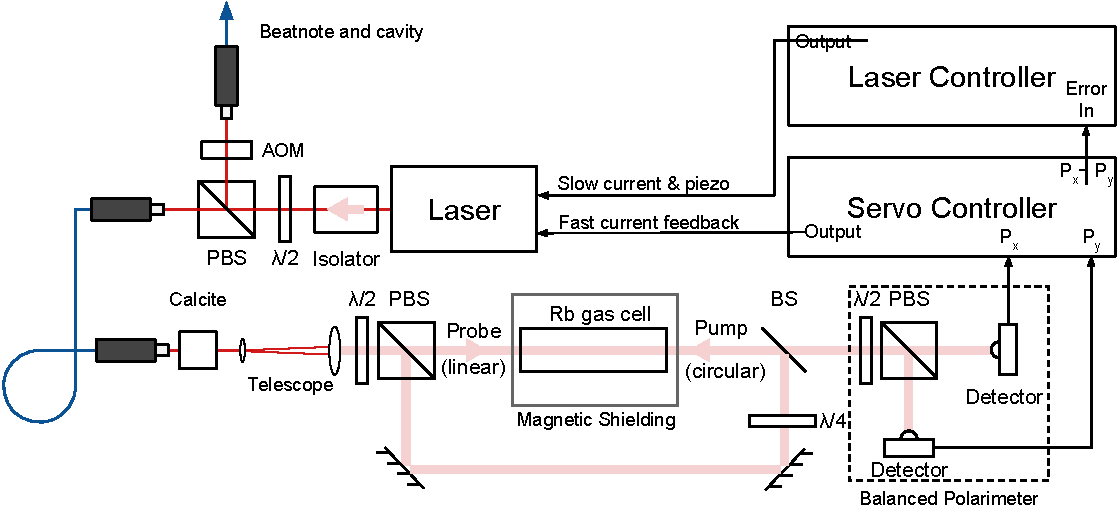
\includegraphics[width=\linewidth]{part1/Figs/fig1.pdf}
\caption{Schematic of a polarization spectroscopy (PS) apparatus.
The beam from the ECDL laser passes through an isolator before being split into two beams by a polarizing beam cube (PBS) and coupled into optical fibers.
One fibre leads to the PS setup and the other to other measurement or experimental apparatus.
The PS setup  consists of a polarization stabilizing calcite prism followed by a beam expanding telescope.
The expanded beam is then divided by a PBS into a linearly polarized probe and circularly polarized pump which counter-propagate, via a non-polarizing 50:50 beamsplitter (BS), through the magnetically shielded atomic gas sample.
The polarization rotation of the probe beam is then measured by a balanced polarimeter which consists of a $\lambda/2$ waveplate, PBS and two detectors.}
\label{polspec_schematic}
\end{figure}

The spectral profile of the difference in absorption coefficients for the circularly polarized components for the atomic medium in the vicinity of a resonance is a Lorentzian with width $\Gamma$, the inverse lifetime of the excited state of the resonant transition~\cite{demtroder_laser_2003}:
\begin{align}
\Delta \alpha = \frac{\Delta\alpha_0}{1+4\left(\frac{\delta}{\Gamma}\right)^2}.
\end{align}
Here $\delta=\omega_L-\omega_A$ is the detuning of the laser from the resonance, $\omega_L$ is the angular frequency of the laser and $\omega_A$ the angular frequency of the atomic resonance.
$\Delta\alpha_0$ is the difference in absorption coefficients for the $\sigma^\pm$ circular polarization components at zero detuning.

The refractive index and absorption of the medium are related through the Kramers-Kronig dispersion relation \cite{demtroder_laser_2003},
\begin{align}
\Delta n = \Delta\alpha_0 \frac{2c}{\omega_A \Gamma}\frac{\delta}{1+4\left(\frac{\delta}{\Gamma}\right)^2}.\label{result}
\end{align}
$\Delta\alpha_0$ is the sum over all $m_F$ ground states of the difference between absorption coefficients for each circular polarization, with $\delta=0$, weighted by the ground ($F, m_F$) and excited state ($F', m_{F\pm1}$) population differences,
\begin{align}
\Delta\alpha_0 = \sum_{m_F=-F}^{+F} \big[\alpha_{(F,m_F\rightarrow F',m_{F+1})}(P_{F,m_F}-P'_{F',m_{F+1}})\nonumber\\
-\alpha_{(F,m_F\rightarrow F',m_{F-1})}(P_{F,m_F}-P'_{F',m_{F-1}})\big].
\end{align}
The absorption coefficient for a given transition is $\alpha_{(F, m_F\rightarrow F',m_{F\pm1})}=N \sigma(\omega_L)$ where $N$ is the total number of interacting atoms, $\sigma(\omega_L)$ is the absorption cross section for the transition and $P_{F,m_F}$ refer to the populations of the various atomic states.

\subsection{Magnetic shielding}

\section{Fast Theory}

\subsection{from paper}
The atomic substate populations can be calculated using \glspl*{obe}~\cite{hughes_polarization_2009} but the standard steady-state solutions provide little insight into the behavior of the error signal when $\delta$ is changing faster than the evolution of the populations.
That evolution is limited to the spontaneous decay rate $\Gamma$, and hence for times $t\ll \tau=1/\Gamma$, the populations can be considered constant.
The \gls*{ps} signal is proportional to the refractive index difference given by Eq.~(\ref{result}), which describes a steep, background-free antisymmetric dispersive function, with bandwidth $1/t$ that can be much greater than $\Gamma$ (Fig.~\ref{sa_ps_spectra}).
Absorption-based frequency stabilization techniques such as \gls*{sa} rely on frequency-dependent changes to the atomic populations, rather than on the refractive index, resulting in dispersive signals over a much smaller capture range, with bandwidth limited to $\Gamma$.
SA is further limited if there are closely spaced hyperfine resonances or cross-over peaks.
Laser frequency noise can extend to frequencies much greater than $\Gamma$, where polarization spectroscopy still provides strong feedback and therefore can achieve much narrower laser linewidth.

\section{OBEs (timescale of state evolution, step in simulating)}

\section{Developments}

\subsection{Balanced Polarimeter}
When Wieman and H\"anch~\cite{wieman_doppler-free_1976} originally described \gls{ps} polarisation rotation was monitored with a nearly crossed polariser as shown in Figure \ref{figure:wieman_doppler-free_schematic}.
The polariser is crossed such that only a small proportion of the probe beam passes through them in the absence of the pump.
With the pump inducing anisotropy the rotation of the probe can be detected after the polarisers.

\begin{figure}
\includegraphics[width=\linewidth]{part1/Figs/wieman_doppler-free_schematic.png}
\caption{Figure stolen from Wieman and H\"anch paper.
Should probably redraw so I'm not plagiarizing.
Or ask how to cite it probably or some such.}
\label{figure:wieman_doppler-free_schematic}
\end{figure}

Pearson et al. proposed the alternative method of using a balanced polarimeter which provides a background-free signal with peak-to-peak height more than an order of magnitude greater than with the crossed polariser method~\cite{pearman_polarization_2002}.

\subsection{Beam splitter to co-propagate}

All papers thus far have ``snuck'' the pump beam through the vapour cell.

Figure with ``snucked'' and beam splitter configuration.

The angle of ``snucking'' has implications that there is math for...

Using a NBPS instead means you have an angle of 0.
The beam splitter has no effect on the polarisation as far as I can tell.

Pumped spectroscopy techniques such as \gls{ps} and \gls{sa}... spectral broadening due to angle stuff.

\subsection{High bandwidth feedback}


\subsection{Lincoln's magic detectors?}

\section{Experimental Setup (with details - fibres, calcite, etc.)}
\subsection{from paper - merge}
Two commercial Littrow configuration \glspl*{ecdl} were individually locked using \gls*{ps}.
The laser beam for each was split by a \gls*{pbs} and propagated through polarization-maintaining fibers to the \gls*{ps} locking system and linewidth measurements.
The locking beams were polarized with Glan-Thompson prisms (Fig.~\ref{polspec_schematic}) to eliminate residual polarization drift in the fibers.
Beam expanding telescopes were used to expand the beam to fill the apertures of the magnetic shielding, approximately \unit[1]{cm} diameter, allowing them to interact with more atoms to increase $|\Delta\alpha_0|$ and improve the \gls*{snr}.

The \gls*{pbs} balanced polarimeter error signal was generated with biased photodiodes (\unit[150]{MHz} bandwidth) and servo controllers (\unit[14]{MHz} bandwidth).
The servo controller integration zero-gain frequency was typically between \unit[100]{kHz} and \unit[1]{MHz}.
The diode modulation could be DC-coupled, with bandwidths of \unit[40]M{Hz} and \unit[10]{MHz}, or AC-coupled, \unit[100]{kHz}\,\textendash\,\unit[40]{MHz} and \unit[10]{kHz}\,\textendash\,\unit[10]{MHz}, depending on the laser.
The laser electronics provided control of the \glspl*{ecdl} piezoelectric transducer and diode injection current, with bandwidths of \unit[1]{kHz} and \unit[50]{kHz} respectively.



\chapter{Measurement Techniques}
We have characterized the performance of \gls*{ps} frequency stabilisation using a number of methods which are detailed here. Spectral linewidth is the principle metric by which stabilisation techniques are compared...

{\color{red}More detail in this intro.}

\section{Heterodyne Methods}

Heterodyning is a technique, invented by Canadian Reginald Feessenden in 1901, which mixes two frequencies to produce a new frequency. {\color{red} [get proper citation, this is from Wiki]} In optics the technique can be used to examine the spectral properties of two lasers.~{\color{red}[Citation?]}

\subsection{Basic Theory}
In the electrical signals context heterodyning involves the `mixing' or multiplying of two sine wave signals to produce two different signals with frequencies equal to the difference and sum of the original frequencies:
\begin{equation}
\sin(\theta_1)\sin(\theta_2) = \frac{1}{2} \cos(\theta_1-\theta_2) - \frac{1}{2} \cos(\theta_1+\theta_2).
\end{equation}

In the optical context this is achieved due to the interference term accrued when squaring the electric field in order to calculate the intensity detected by the photodetector. The intensity of an electric field is given by:
\begin{equation}
I(t) = \frac{c\epsilon_0}{2}|E|^2.
\end{equation}

For two copropagating lasers with electric fields $E_{1, 2}$ and angular frequencies $\omega_{1, 2}$ we can write
\begin{equation}
E_{1, 2}(t) = \sin(2\pi \omega_{1, 2}).
\end{equation}
The electric field at the detector, $E_T$, is given by the sum of $E_{1,2}$, such that
\begin{align}
I(t) &= |E_1(t) + E_2(t)|^2\nonumber\\
&= E_1(t)^2 + E_1(t)E_2(t) + E_2(t)^2.
\end{align}
The interference, $E_1(t)E_2(t)$, term allows heterodyning of optical signals.

\subsection{Optical Heterodyne Methods}

There are a number of linewidth measurement techniques that utilise heterodyning. The major ones are:
\begin{itemize}
\item Heterodyne beatnote with two identical lasers.
\item Heterodyne beatnote between laser of interest and a relatively narrow reference laser.
\item Self-heterodyne beatnote of a laser with itself.
\end{itemize}

\subsection{Linewidth Discrepancies}
There is an interesting discrepancy between intuition and what the literature uses to describe `linewidth'.
Intuitively, when discussing the spectral properties of light, one would expect references to refer to the properties of the electric field since that is the entity that is interacting with atoms and other frequency references.
However, the literature seems to exclusively refer to properties of the power of the signal from photodetectors, as shown on spectrum analysers, which differ by a factor of 2 which will be shown below.
Despite this fact this document follows the convention to avoid confusion.

The simplest way to examine a heterodyne signal is to look at the signal from the detector on a radio-frequency spectrum analyser.
A spectrum analyser shows the power for each frequency component of the input electrical signal.
The power of the electrical signal from the detector, $P_{elec}$ is roughly:
\begin{equation}
P_{elec}\propto I^2 \propto E^2
\label{eq:beatnote_proportional}
\end{equation}
where $I$ is the light intensity incident on the detector and $E$ is the electric field incident on the detector.

Of primary interest are the spectral properties of these signals which are given by their Fourier transform.
However we cannot simply write
\begin{equation}
\mathcal{F}[P_{elec}]\propto \mathcal{F}[I^2] \propto \mathcal{F}[E^2]
\end{equation}
since it's not true.
The inverse convolution theorem, however, can be used
\begin{equation}
f\cdot g = \mathcal{F}^{-1} \bigg[ \mathcal{F}[f] \otimes\mathcal{F}[g]\bigg].
\end{equation}

So Eq. \ref{eq:beatnote_proportional} in Fourier space becomes
\begin{align}
\mathcal{F}[P_{elec}]&\propto \mathcal{F}[I]\otimes\mathcal{F}[I]\nonumber\\
&\propto \big\{\mathcal{F}[E] \otimes\mathcal{F}[E]\big\} \otimes\big\{\mathcal{F}[E] \otimes\mathcal{F}[E]\big\}
\end{align}

For a Gaussian lineshape beatnote with \gls{rms} width $\sigma$, we can write
\begin{equation}
\mathcal{F}[E] = A e^{-(f-f_0)^2/2\sigma^2}.
\end{equation}

It is easy to show that the convolution of two Gaussians produces another Gaussian with variance equal to the sum of the variance of the two constituent functions.
Thus,
\begin{equation}
\mathcal{F}[I] = B e^{-(f-f_0)^2/4\sigma^2}
\end{equation}
and
\begin{align}
\mathcal{F}[P] &= B e^{-(f-f_0)^2/8\sigma^2}\nonumber\\
&= B e^{-(f-f_0)^2/2(2\sigma)^2}
\end{align}
So the width of the signal shown on a spectrum analyser has twice the spectral width of the electric field that generated it.

\begin{figure}
\centering
\includegraphics[width=0.5\linewidth]{part1/Figs/beatnote.jpg}
\caption{Depiction of simple beatnote.}
\label{figure:simple_beatnote}
\end{figure}

\subsection{Self-heterodyne}

Self-heterodyne is...

Single delay...

How much delay?

Multipass delay...

These are the results I got...

They look good... too good.

Here's why...\cite{richter_linewidth_1986}

\section{Frequency Reference}
\begin{itemize}
\item Identical laser
\item Narrow laser
\item Three Gaussian lasers
\end{itemize}

\subsection{from paper - merge}
To investigate the discrepancy between the two laser linewidth measurements we used heterodyne measurements which are insensitive to amplitude noise.
Heterodyne measurements were made by frequency shifting one of the laser beams with a double-pass \gls*{aom} and combining the two locked beams on a 50:50 beamsplitter followed by a \unit[1]{GHz} bandwidth photodetector.
The beatnote spectrum was measured with a radio frequency spectrum analyzer, see Fig.~\ref{beatnote}.
Most of the optical power is within the central peak of the spectrum, with \unit[-3]{dB} full width of \unit[$2.0\pm1.1$]{kHz} determined from a Gaussian fit.
The lasers are uncorrelated and if they have identical, Gaussian lineshapes then the single laser \gls*{rms} linewidth is \unit[$0.60\pm0.32$]{kHz}.
The shoulders in the spectrum around \unit[$\pm1.5$]{MHz} correspond to the servo bump of the fully locked spectra in Fig.~\ref{fig:PSDs}.

{\color{red} Rob to determine single laser linewidth from \unit[-3]{dB} beatnote width}

\begin{figure}[htbp]
\centering
\includegraphics[width=\linewidth]{part1/Figs/fig5_v1.pdf}
\caption{Heterodyne beatnote for the two lasers locked with \gls*{ps}.
The inset figure is a higher resolution measurement of the central peak with a Gaussian fit (red), \unit[-3]{dB} width of \unit[2.0$\pm$1.1]{kHz}.
Both figures are 50 shot averages with resolution bandwidths of \unit[30]{kHz} and \unit[100]{Hz} and total measurement times of approximately \unit[0.5]{s} and \unit[2]{s} respectively.}
\label{beatnote}
\end{figure}

\begin{table}[htbp]
\centering
\begin{tabular}{c c c}
\hline
  & Method & RMS Linewidth (kHz) \\ \hline
  (i) & Cavity transmission mapping  & $2.0 \pm 0.4$ \\
  (ii) &Cavity transmission integral & $2.4 \pm 1.0$ \\
  (iii) & Heterodyne & $0.60\pm0.32$ \\ \hline\end{tabular}
\caption{Linewidth results.
(i) Mapping the transmission signal through a cavity with a \gls*{fwhm} of \unit[71.6]{kHz} to a Lorentzian signal followed by deconvolving from the amplitude noise.
(ii) The results from integrating the power-spectral density of the cavity transmission signal (Fig.~\ref{fig:PSDs}) (iii) The heterodyne beatnote (Fig.~\ref{beatnote}).}
\label{linewidth_table}
\end{table}

\section{Noise measurements}
\subsection{From paper - merge}
\begin{figure}[htbp]
\centering
    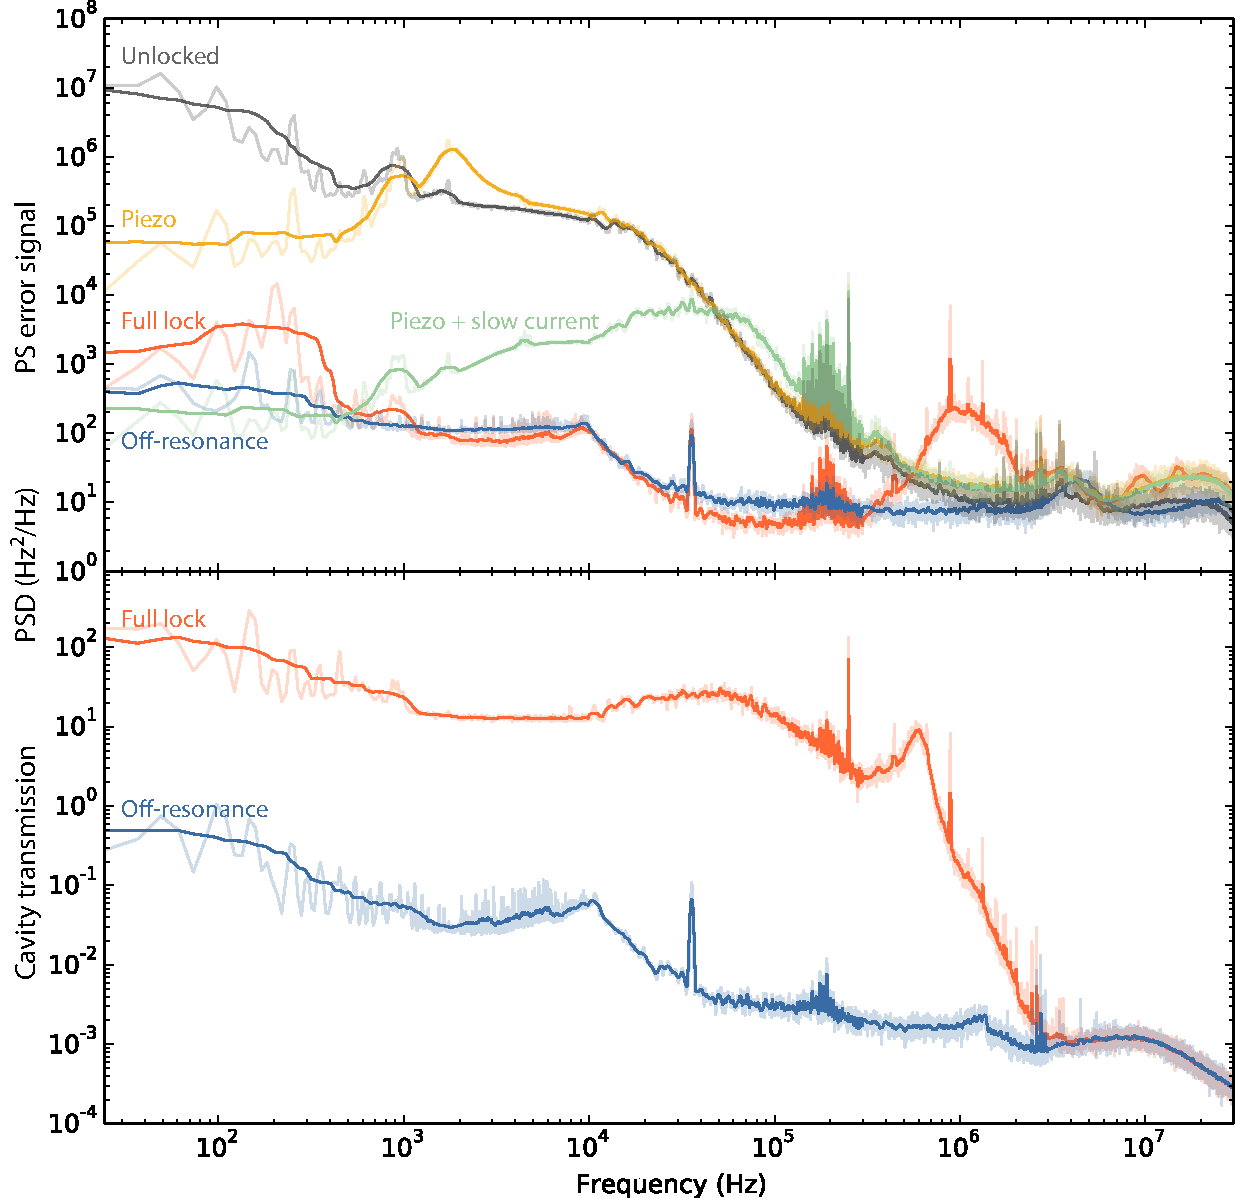
\includegraphics[width=0.9\linewidth]{part1/Figs/fig4a_v3.pdf}
    \label{fig:PSDs}
    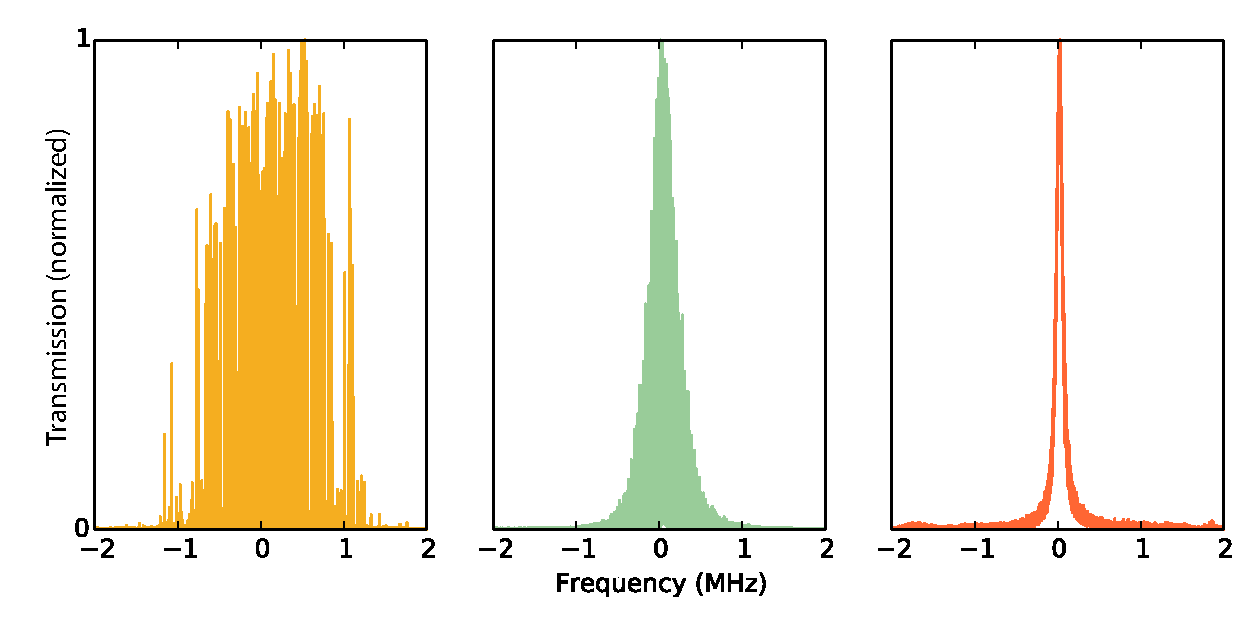
\includegraphics[width=0.9\linewidth]{part1/Figs/fig4b_v1.pdf}
    \label{fig:cavity_scans}
\caption{Frequency noise measurements.
(a) \Gls*{psd} of polarization spectroscopy error signals for a range of laser locking regimes with laser on resonance: unlocked; piezo-only feedback; slow current and piezo feedback; piezo, slow current, and fast AC-coupled current feedback; the noise floor of the noise measurement with no light on the \gls*{ps} detectors.
Laser power \unit[6.5]{mW}.
The measurements are shown with a superposed smoothed curve (moving average  with window size $10\log_{10}(f)$ where $f$ is the frequency).
(b) Optical cavity transmission as a function of laser offset frequency for locking with varying bandwidth.
Piezo only (left), piezo and slow current (middle) and piezo, slow current and fast current (right).
Cavity \gls*{fwhm} linewidth \unit[71.6]{kHz}, scan time \unit[100]{ms}, laser power \unit[170]{$\mu W$}.
(c) \Gls*{psd} of transmitted cavity signal at half peak height for the piezo, slow current and fast AC-coupled current feedback.
For (a) and (c) noise below \unit[$10^4$]{Hz} was measured with a high dynamic range audio digitizer with a resolution bandwidth (RBW) of \unit[12]{Hz}; an RF spectrum analyzer was used at higher frequencies, with RBW of \unit[30]{Hz} between \unit[$10^4$]{Hz}\textendash\unit[$10^6$]{Hz} and RBW of \unit[300]{Hz} above \unit[$10^6$]{Hz}} 
\end{figure}

\subsection{Error Signal Noise}
The spectrum of the \gls*{ps} error signal provides a measure of the laser frequency noise in combination with the \gls*{ps} frequency discrimination, photodetector and electronic noise and gain.
The response of the system to different feedback parameters and the underlying noise limitations are immediately apparent.
The frequency noise \glsfirst*{psd} of the \gls*{ps} error signal (Fig.~\ref{fig:PSDs}) was measured for different feedback configurations, using a high-dynamic-range audio digitizer (low frequency, \unit[\textless10]{kHz}) and radio-frequency spectrum analyzer (high frequency, \unit[10]{kHz} to \unit[30]{MHz}).
The spectrum analyzer was calibrated using the slope of the error signal at resonance.
The low frequency data were calibrated by matching to the spectrum analyzer data at \unit[10]{kHz}.  

Increasing suppression of noise is readily apparent as the feedback bandwidth is increased from \unit[1]{kHz} (piezo only) to \unit[50]{kHz} (piezo and slow current through the laser controller) and then full lock with feedback via direct diode current modulation.
From around \unit[450]{Hz} to \unit[350]{kHz} the fully locked noise spectrum is coincident with the noise floor measured by detuning the laser far from resonance, and intersects with the unlocked spectrum at \unit[700]{kHz}.
A servo bump peaked at \unit[1.3]{MHz} is consistent with a phase lag in laser diode response to current modulation~\cite{wieman_using_1991}.

\subsection{Cavity Transmission Noise}
The error signal spectra provide useful information for optimising the locking system to reduce the laser frequency noise spectrum.
To measure the laser frequency noise spectrum itself we used a high-finesse optical cavity as an independent laser frequency discriminator.
With finesse of 20942 and free spectral range of \unit[1.50]{GHz}, the optical cavity had \gls*{fwhm} linewidth of \unit[71.6]{kHz}.
Fig.~\ref{fig:cavity_scans} shows cavity transmission signals as the laser frequency incident on the cavity was scanned with a double-pass \gls*{aom}.
The resulting traces provide a clear illustration of the effect of increased locking bandwidth: with piezo-only locking the peak appears broad as the laser jitters around the resonant frequency.
With slow current feedback, the transmission peak shape becomes apparent, and finally we see the effect of high-bandwidth feedback with peak width limited by the cavity finesse, indicating a laser linewidth much smaller than the cavity linewidth.

We analyzed the frequency noise of the laser through the cavity transmission signal by choosing a static \gls*{aom} frequency such that the transmitted power through the optical cavity was half the peak power, where the transmission-frequency response is approximately linear. 

The cavity noise spectrum is shown in the lower portion of Fig.~\ref{fig:PSDs} for full bandwidth AC-coupled locking.
The signal was well above the noise floor, measured with laser frequency between transmission peaks, for frequencies up to the \unit[5.5]{MHz} bandwidth of the photodetector.
 This approach could not be used with lower-bandwidth feedback because the laser linewidth was wider than the cavity transmission.
 Note that the cavity transmission noise floor is three to four orders of magnitude lower than that of the \gls*{ps} error signal, in part due to the much lower laser power (microwatts rather than milliwatts) and hence lower shot noise.

We extracted a measure of the linewidth from the cavity data using two methods: first we mapped the amplitude noise of the locked cavity signal to frequency using the cavity transmission frequency response shown in Fig.~\ref{fig:cavity_scans}.
The standard deviation of the distribution of frequencies gave an \gls*{rms} linewidth of \unit[2.4$\pm$0.4]{kHz}.
We also integrated the power spectral density to find an RMS linewidth \cite{negnevitsky_wideband_2013} of \unit[2.4$\pm$1.0]{kHz}.
Linewidth results are summarized in Table \ref{linewidth_table}.

The cavity transmission spectra and linewidth measurements include contributions from both laser frequency and amplitude noise.
An estimate of the amplitude noise contribution to the spectra was obtained by measuring the photodetector power spectrum without the cavity and thus without frequency noise, with the same incident laser power on the photodetector.
Mapping that noise spectrum to frequency produced a contribution of \unit[1.4$\pm$0.3]{kHz} in the cavity transmission mapping linewidth,  and \unit[0.16$\pm$0.07]{kHz} to the PSD integral linewidth.
As expected, the cavity transmission mapping method is more susceptible to laser amplitude noise. 

Assuming the measurements are uncorrelated convolutions of the frequency and amplitude noise contributions, the linewidth determined from cavity transmission mapping consists of the \unit[1.4$\pm$0.3]{kHz} amplitude noise linewidth in combination with a frequency noise linewidth of \unit[2.0$\pm$0.7]{kHz}.
The difference is likely because the mapping method does not properly include contributions from higher Fourier frequencies; that is, the ``pedestal'' of the laser spectrum which can be seen in a heterodyne measurement.

\section{Side of peak (include basic cavity theory here?)}
\section{Integration}
\section{Measuring Slow Frequency Drifts}
\subsection{to merge}

Polarization spectroscopy is inherently a DC technique, susceptible to low frequency drift ($1/f$ noise).
Drift in the laser power output as the laser alignment drifts, variations in fiber coupling efficiency if fibers are used, variations in the atomic vapor density due to changes in temperature, thermal effects on the waveplates and changes to the electronic gains and offsets can all affect the lock point of PS due to the resulting intensity noise combined with the difficulty in perfectly balancing the polarimeter.

The high-finesse cavity was used as a reference to quantify the long-term drift of the PS locked laser over a period of 60 hours (fig.~\ref{fig:drift}).
Drift in the optical cavity frequency was corrected by reference to a laser AC-locked to the rubidium transition using saturated absorption.
The standard deviation of the PS-locked laser frequency measurements was 51\,kHz, approximately half the standard deviation of the measurements in Ref.~\cite{tiwari_laser_2006} and significantly smaller than the 400\,kHz quoted in Ref.~\cite{lee_frequency_2014}.
The frequency change between 10\,s measurements was on average 5\,Hz, with a standard deviation of 210\,Hz.

\begin{figure}[htbp]
\centering
\includegraphics{part1/Figs/drift.pdf}
\caption{Frequency drift of a polarization spectroscopy locked laser, in units of natural linewidth $\Gamma$ and MHz, over a 60 hour period measured every 10 seconds.
The standard deviation of the frequency measurements was 51\,kHz.}
\label{fig:drift}
\end{figure}

The frequency stability of PS is strongly dependent on the extent to which the apparatus is isolated from ambient temperature variations~\cite{yoshikawa_frequency_2003}.
In our system the lasers are temperature stabilized and isolated with acrylic enclosures, and the optical cavity was temperature controlled and isolated inside a vacuum chamber, but the PS and SA components and optical components between lasers and optical cavity were not temperature controlled or shielded from the general laboratory environment.
The locking stability and drift are expected to improve with environmental isolation of all optical components and temperature stabilization of the atomic vapor cell.
The power into the PS setup is particularly sensitive to polarization drift in the light exiting the optical fibers.
Although singlemode polarization maintaining fibers were used, they exhibited significant polarization drift with laboratory temperature variations, and we expect shielded free-space propagation or active power stabilization of the light into the PS setup would further improve the frequency stability.

\section{Bandwidth Stuff}
\subsection{From paper - merge}
\label{bandwidth_section}
The capture range and bandwidth of the frequency discriminator are important in determining the ultimate linewidth that can be achieved, and the ability to compensate for sudden disturbances to the laser frequency, for example due to external shock or vibration.
We define the capture range as twice the minimum frequency difference from resonance for which the locking signal is of the correct sign for negative feedback, which can be deduced from the error signal by locating the first zero crossing to either side of the resonance.
For the spectra shown in Fig.~\ref{sa_ps_spectra} this is greater than \unit[300]{MHz}, many times larger than the \unit[16]{MHz} of \gls*{sa}, as shown in Fig.~\ref{sa_ps_spectra}.

The frequency noise spectrum of the \gls*{ps} error signal is shown in  Fig.~\ref{bandwidth}, both on-resonance and with laser far detuned to determine the noise floor.  The signal and noise intersect at \unit[83]{MHz}.
Since the sign of the \gls*{ps} error signal is constant over that range (see fig.~\ref{sa_ps_spectra}), the \unit[83]{MHz} noise-limited signal bandwidth is indicative of the high bandwidth available from polarization spectroscopy.
In contrast, the \gls*{sa} signal reverses sign several times within \unit[83]{MHz}, and the effective bandwidth is limited by the \unit[$\pm 8$]{MHz} capture range of \gls*{sa}.

\begin{figure}[htbp]
    \centering
    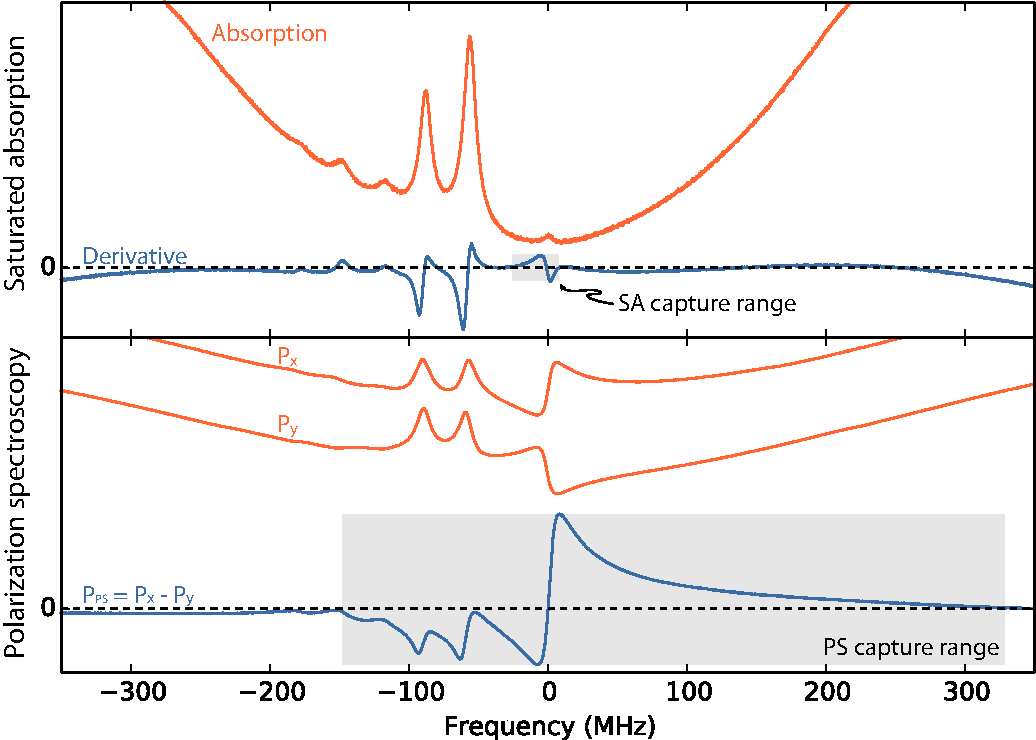
\includegraphics[width=\linewidth]{part1/Figs/fig2_v1.pdf}
    \caption{Saturated absorption spectroscopy (SA) and polarization spectroscopy (PS) spectra for the $^{85}$Rb D2 transition.
The upper portion of the figure shows the absorption and error spectra for SA.
The lower portion shows the components of the PS error signal ($P_{x,y}$ in Fig. \ref{polspec_schematic} and Eq. \ref{P_PS}) and the PS error signal.
The shaded regions indicate the approximate capture range of the respective error signals.
Zero frequency at $^{85}$Rb, $5^2S_{1/2} F=3\rightarrow5^2P_{3/2} F=4$ transition.
Absorption signals normalized to the same maximum absorption on resonance.}
    \label{sa_ps_spectra}
\end{figure}

\begin{figure}[hbp]
    \centering
    \includegraphics[width=\linewidth]{part1/Figs/fig3_v1.pdf}
    \caption{Polarization spectroscopy error signal frequency noise spectra.
Upper trace (black): frequency spectrum of the error signal while the laser is unlocked and centered on the $^{85}$Rb 5$^\text{2}$S$_\text{1/2}$ $\rightarrow$ 5$^\text{2}$P$_\text{3/2}$ transition.
Lower trace (red): spectrum with laser far from resonance.
The two lines intersect at approximately \unit[83]{MHz}.
Laser power \unit[7.5]{mW} after isolator, with pump:probe ratio 1.4.
The measurements are shown with a superposed smoothed curve (moving 20-point average).}
    \label{bandwidth}
\end{figure}

\section{Long Term Stability}
\subsection{from paper - merge}
Polarization spectroscopy is inherently a DC technique, susceptible to low frequency drift ($1/f$ noise), for example drift in the laser power output as the laser alignment drifts, variations in fiber coupling efficiency, variations in the atomic vapor density due to changes in temperature or local magnetic field, or changes to the electronic gains and offsets.
To quantify the long-term stability, the beatnote between a \gls*{ps}-locked laser and a laser locked to an \gls*{sa} peak was tracked over a number of days.
The \gls*{sa} laser was AC-locked using FM demodulation; that is, with current modulation at \unit[250]{kHz} and demodulation of the detected signal.
FM modulation is inherently insensitive to many of the slow variations that can affect the lock frequency, so that variations in the beatnote frequency can be attributed to the drift in the \gls*{ps} laser.
A linear fit to the beatnote data (Fig.~\ref{drift}) sets an upper limit on the frequency drift of less than \unitfrac[2]{kHz}{h}. 

Others have measured drifts of \unitfrac[17]{kHz}{h} to \unitfrac[1]{MHz}{h}~\cite{yoshikawa_frequency_2003, tiwari_laser_2006} and standard deviation of \unit[400]{kHz} \cite{lee_frequency_2014}, depending on the extent to which the apparatus was isolated from ambient temperature variation.
In our system the lasers are temperature stabilized and isolated from the environment with acrylic boxes, but the \gls*{ps} and \gls*{sa} components were not temperature controlled or shielded from the general laboratory environment.
Polarization and power stabilization of the laser, and temperature stabilization of the atomic vapor cell, are likely to improve the locking stability and drift.

\begin{figure}[htbp]
\centering
\includegraphics[width=\linewidth]{part1/Figs/fig6_v1.pdf}
\caption{Measurement of frequency drift of a polarization spectroscopy locked laser over a 50 hour period.
Upper: frequency deviation and linear fit with gradient \unitfrac[-1.7]{kHz}{h} sets an upper limit to the drift.
The standard deviation of the frequency measurements, acquired at \unit[5]{min} intervals, was \unit[155]{kHz}.
Lower: temperature (dotted line) and pressure (dashed line) of the laboratory over the same period of time, measured every \unit[200]{ms}.}
\label{drift}
\end{figure}

\section{Conclusion}
We have demonstrated laser frequency stabilization using a polarization spectroscopy reference, and reduced the linewidth of \gls*{ecdl} lasers well below \unit[1]{kHz}, much lower than previously demonstrated with this technique and previously achieved only by locking to high-finesse optical cavities.
The absolute frequency drift of less than \unit[50]{kHz} per day is adequate for many laser cooling experiments.
Further improvements to drift could be achieved with simple measures such as temperature stabilization and environmental isolation.
The experimental setup provides an approach with low complexity and low cost, providing wide bandwidth linewidth narrowing without radio frequency modulation while retaining an absolute atomic reference.

In our experiments, the locking bandwidth is limited by the phase lag in the laser diode response to injection current variation, to around \unit[700]{kHz}.
With appropriate servo loop shaping, for example multiple phase lead stages to compensate for the diode response, it is reasonable to expect a bandwidth increase to several MHz.
However, the effect on linewidth would be negligible because the \gls*{ps} signal-to-noise ratio is small in this frequency range.
Much greater improvements could be made by lowering the \gls*{ps} noise floor, which is three to four orders of magnitude higher than the noise floor of the optical cavity.
The difference is only partly due to the $100\times$ higher power in \gls*{ps}, which will increase shot and Johnson noise by $10\times$.
 More...



\part{Evolution of the Cold-Atom Electron Source}

Chapters should be split in to separate files when I'm satisfied with the vague plan.

\chapter{Introduction}

\section{Diffractive Imaging}

\subsection{Crystallography etc}

\section{Coherent Diffractive Imaging}

\section{Cold-Atom Electron Sources}




\chapter{Cold-Atom Electron Source}\label{chapter:setup}

\section{Properties}

\section{How it works}

\label{section:two_stage_ionisation}
\label{section:excess_energy}
\label{section:pulse_blaster}

\section{Current Limitations}

\section{Pulsed vs Continuous}

\subsection{Oven Temperature to Electron Count}

\section{Stability}\label{section:stability}

\section{Source Characterisation}

\subsection{Astigmatism}

\subsubsection{Quadrupole Correction}\label{section:quadrupole}

\subsection{Emittance Measurements}

\subsection{Streaked emittance}

\subsection{Coherence}

\subsection{Noise characterisation}

\section{Future Ideal source}


\chapter{Ultrafast Diffractive Imaging}

\section{Theory}

\section{Why ultrafast?}

\section{How does CAES do it?}

\section{Results}

\subsection{Gold}

\subsection{Aluminium}

\subsection{Graphene}

\subsection{Other Stuff}

\section{Why don't all our samples work?}


\chapter{Time-Resolved Emittance Measurements}

\section{Introduction}

\subsection{What is Emittance}
 

\subsection{What Emittance is useful for}

\section{Theory}

A given ensemble of particles can be described by its density in six-dimensional phase space, $(x, p_x, y, p_x, z, p_z)$ where $(x, y, z)$ are the positions and $(p_x, p_y, p_z)$ are the momenta of each particle.
The extent of the beam in phase space is called the \emph{emittance} of the beam.
Each cartesian direction is usually examined separately, $(x, p_x)$, $(y, p_y)$ and $(z, p_z)$ where $z$ is the optic axis of the beam.

Typically the gradients of trajectories in $x$-$z$ and $y$-$z$ are measured rather than the momenta.
These gradients are referred to as the divergence and are defined as $x^\prime \equiv \frac{dx}{dz} = \frac{v_x}{v_z}$.
The space of $(x, x^\prime)$ is referred to as trace-space. The \emph{emittance} can be defined as
\begin{equation}
\epsilon^x \equiv \frac{A^x}{\pi}
\end{equation}
where $A^x$ is the area occupied by the beam in trace space.

The density, $\rho$, of a beam of $N$ particles in trace space can usually be described by a Gaussian:
\begin{equation}
\rho(x, x^\prime) = N exp\left[ \frac{-(\sigma_{22}x^2-2\sigma_{12}xx^\prime+\sigma_{11}x^{\prime2}}{2|\sigma|} \right]
\end{equation}
where $|\sigma|$ is the determinant of the symmetric beam matrix,
\begin{equation}
\sigma = \begin{pmatrix} \sigma_{11} & \sigma_{12} \\ \sigma_{21} & \sigma_{22} \end{pmatrix}
\end{equation}
$\sigma_{11}$ is the standard deviation of $x$, $\sigma_{22}$ the standard deviation of $x^\prime$ and $\sigma_{12}=\sigma_{21}$ indicates the coupling between $x$ and $x^\prime$. The \emph{emittance} can also be defined as
\begin{equation}
\epsilon^x \equiv \sqrt{|\sigma|} = \sqrt{\sigma_{11}\sigma_{22}-\sigma_{12}^2}
\end{equation}

The \emph{\gls{rms} emittance} of the ensemble can be defined as
\begin{equation}\label{emittance}
\epsilon \equiv \sqrt{\langle x^2\rangle \langle x^{\prime 2}\rangle - \langle x x^\prime\rangle^2}.
\end{equation}

\section{Measurement}

Directly calculating the emittance of an ensemble with Eq. \ref{emittance} requires full knowledge of the position and momenta of the particles which is difficult since beam monitors tend to only measure the transverse positions of particles.
There are a number of methods to practically calculate the emittance of a particle beam, namely pepperpots, the multiple profile method methods and the quadrupole method.

\subsection{Pepperpots}

\subsection{Multi-profile Method}
The multi-profile method involves measuring the profile of the beam at a minimum of three locations along the propagation axis.


\subsection{Quadrupole Method}

\section{Simulation}



\subsection{Pepperpots}

\subsection{Multiple Profile Method}

\subsection{Quadrupole Method}

\subsection{Streaking}

\subsection{Experimental Setup}

\subsubsection{Electron Energy}

\subsubsection{Flux}

\section{Samples}

\section{Results}


\chapter{Conclusion}

Where do we go from here?

\section{Why CDI won't work with this generation of CAES}

\section{New source}

\section{What can the old source investigate?}




\appendix
\chapter{Glossary}
\printglossary

% References
%\bibliographystyle{unsrt}
%\renewcommand\bibname{References}
\printbibliography

\end{document}
